\section{Data}
\begin{frame}{Data}
    \vspace{-0.35cm}
    \begin{figure}
        \centering
        \includegraphics[width=1\linewidth]{Figures/pipelineData.pdf}
        \label{fig:pipelineData}
    \end{figure}
    \label{frame:pipelineData}
\end{frame}

% surface features rausnehmen, protein crystallization kürzer fassen, esm kürzer fassen, slide 17 raus, prostT5, data study (und conclusion auf die slides conclusion auf die slides packen), verbal struktur verbessern
\subsection{Crims}
% animate points with images to make clearer 
% add loss function to slide and remove 
\begin{frame}{Crims}
    \begin{columns}[T]
        \column{0.7\textwidth}
        \begin{itemize}[<+->]
            \item local  $\rightarrow$ low protein variance
            \item high-quality crystallization dataset with \textbf{both positive \& negative outcomes}
            \item \textbf{804 plate--shelf combinations}, conditions, and time points (\textbf{619k images})
            \item Protein sequences and shelf-specific variants had to be \textbf{manually reconstructed} $\rightarrow$ main source of uncertainty
        \end{itemize}
    \vspace{-0.4cm}
    \begin{figure}[t]
        \centering
        % Row 1
        \only<3->{
        \begin{subfigure}[b]{0.3\textwidth}            
            \includegraphics[width=\textwidth]{media/FORMULATRIX_SD30010705_2_01-10-2025_05_06_01_00_99_Vis}
        \end{subfigure} \hspace{0.01cm}% <---- reduce horizontal space
        \begin{subfigure}[b]{0.3\textwidth}
            \includegraphics[width=\textwidth]{media/FORMULATRIX_SD30010705_2_01-10-2025_04_06_01_00_99_Vis}
        \end{subfigure}
        \begin{subfigure}[b]{0.3\textwidth}
            \includegraphics[width=\textwidth]{media/FORMULATRIX_SD30010705_2_01-10-2025_03_06_01_00_99_Vis}
        \end{subfigure}			
        }
        \label{fig:crystallization_drops_example_no_scores}
    \end{figure}

        \column{0.3\textwidth}
        \vspace{-0.8cm}
        \begin{figure}
		\centering
        \only<2->{
		\includegraphics[width=1\linewidth]{Figures/CrimsScreenShot.png}}
		\label{fig:crimsScreenshot}
	    \end{figure}
    \end{columns}
\end{frame}

\begin{frame}{Crims Annotation Pipeline}
    \begin{columns}[T]
        \column{0.6\textwidth}
        \begin{figure}[t]
            \centering
            % Row 1
            \begin{subfigure}[b]{0.24\textwidth}
                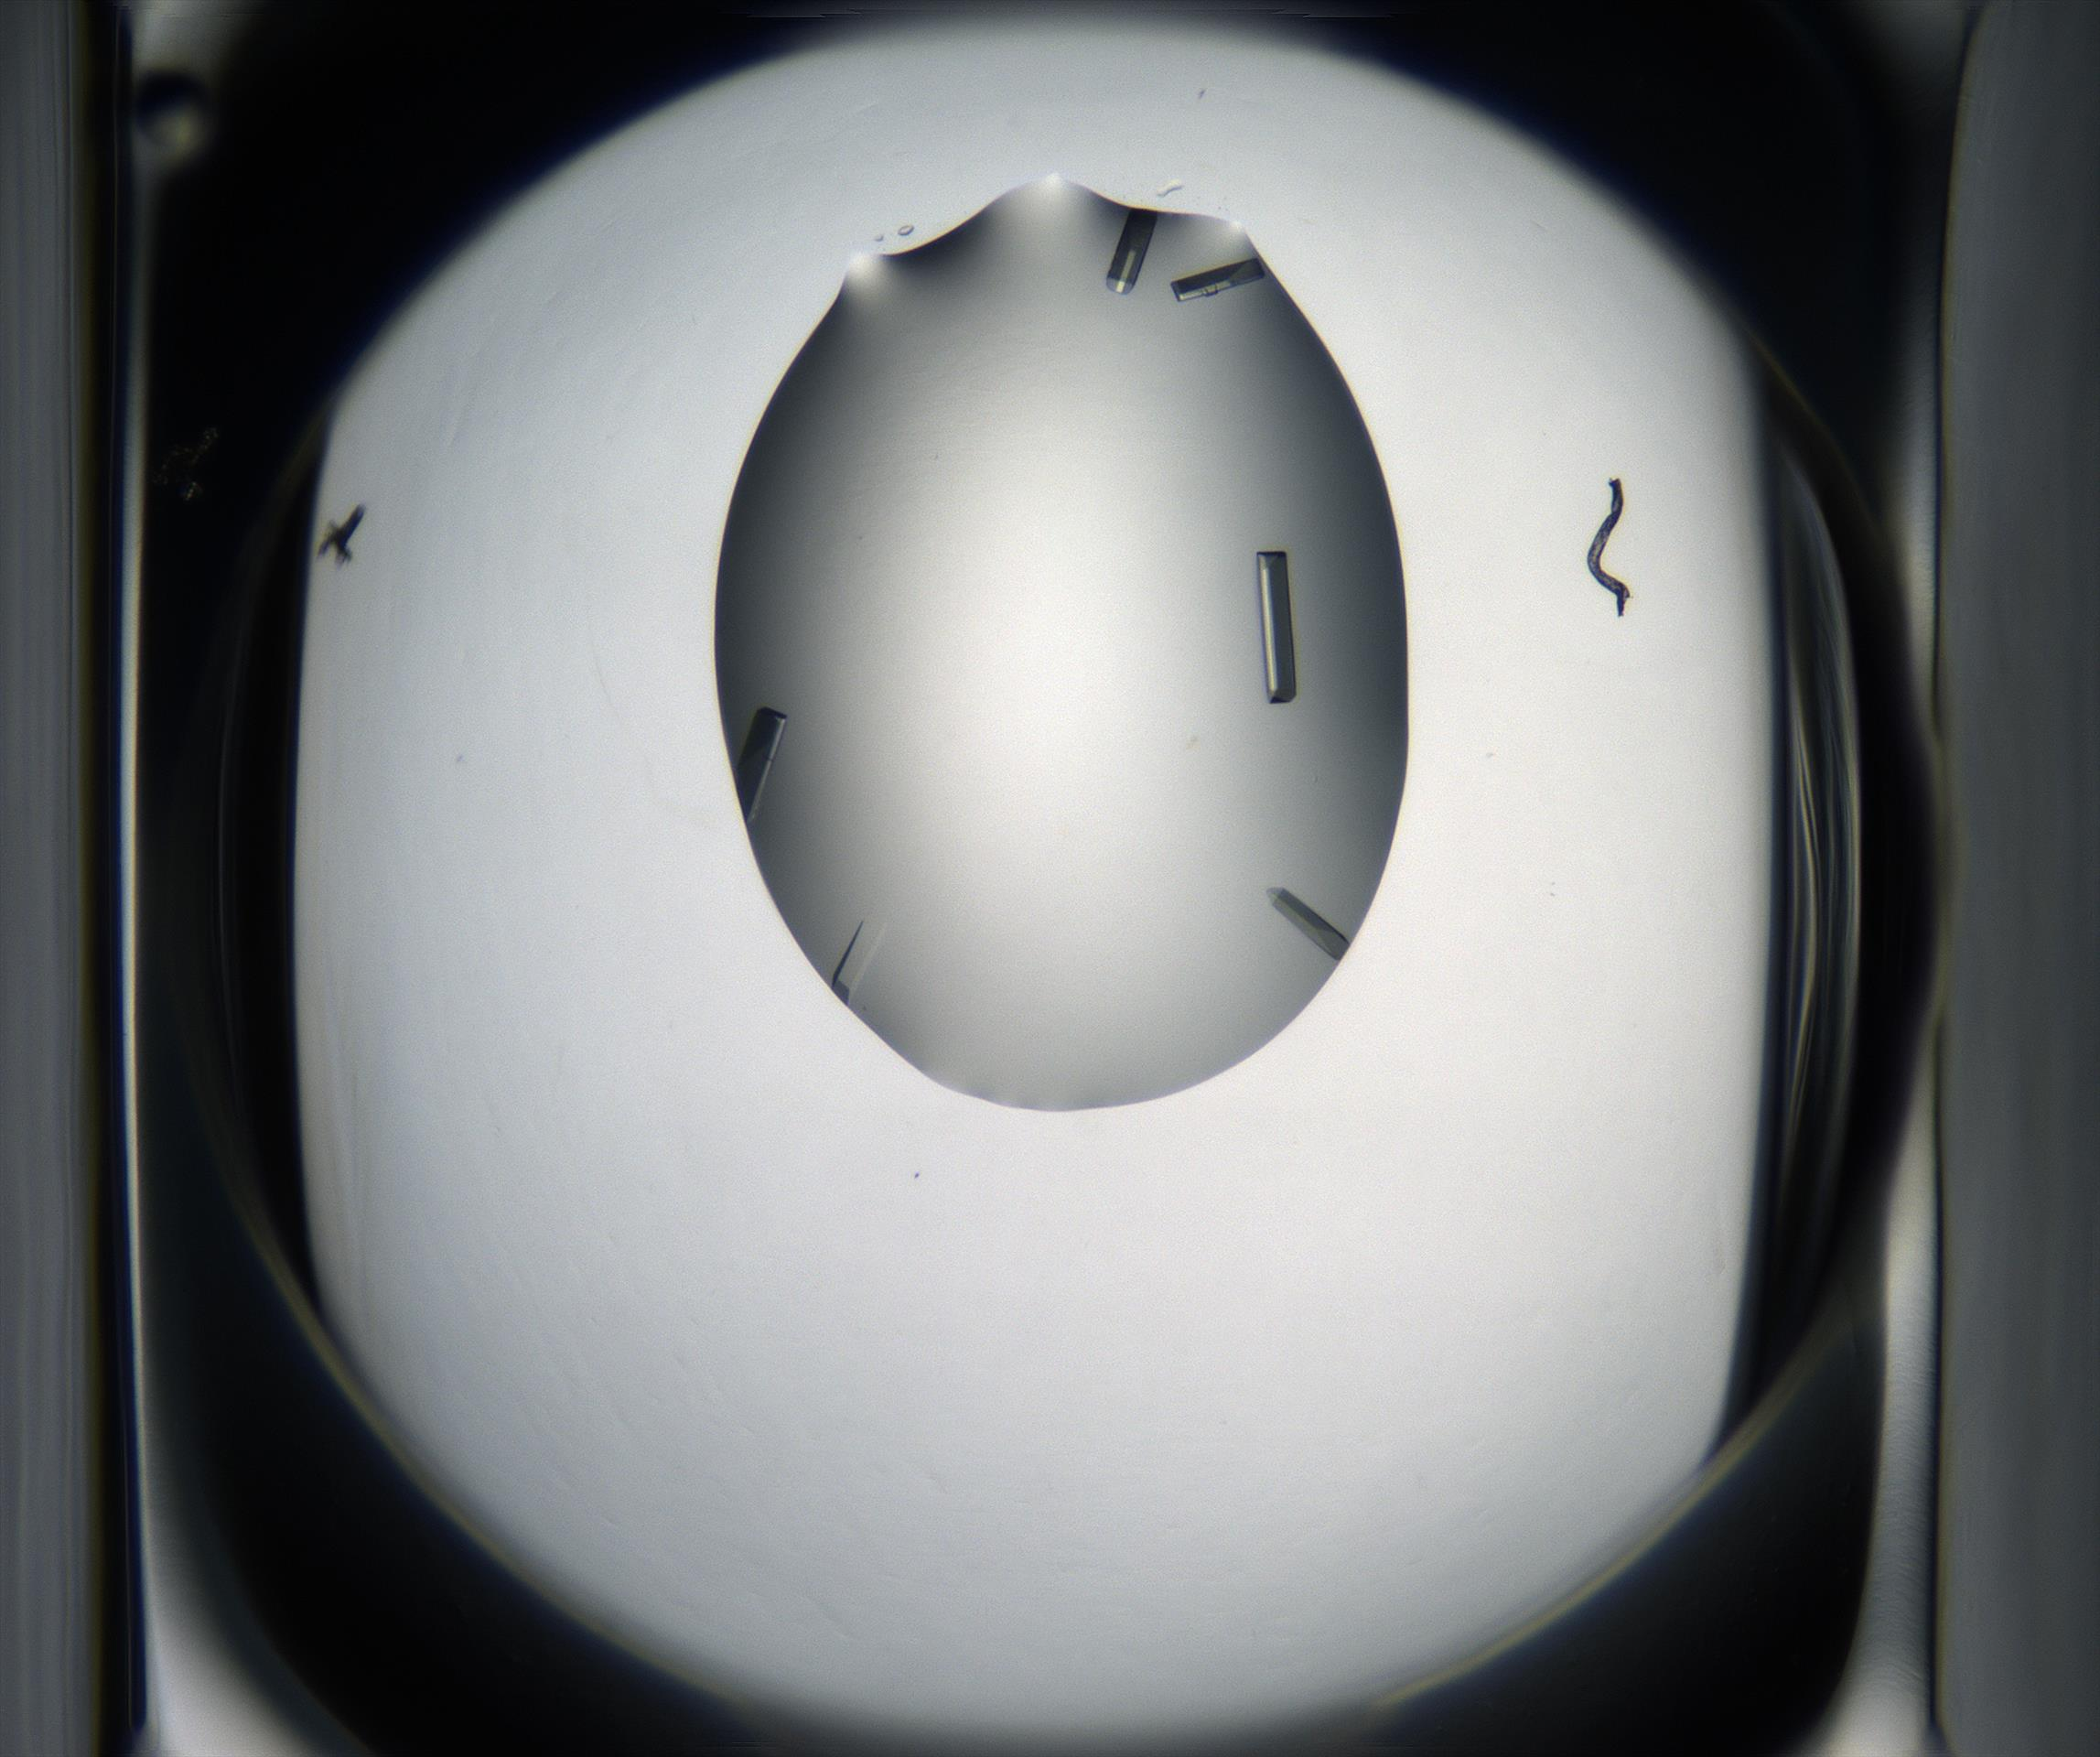
\includegraphics[width=\textwidth]{media/FORMULATRIX_SD30010705_2_01-10-2025_03_03_01_00_99_Vis-1}
            \end{subfigure} \hspace{0.01cm}% <---- reduce horizontal space
            \begin{subfigure}[b]{0.24\textwidth}
                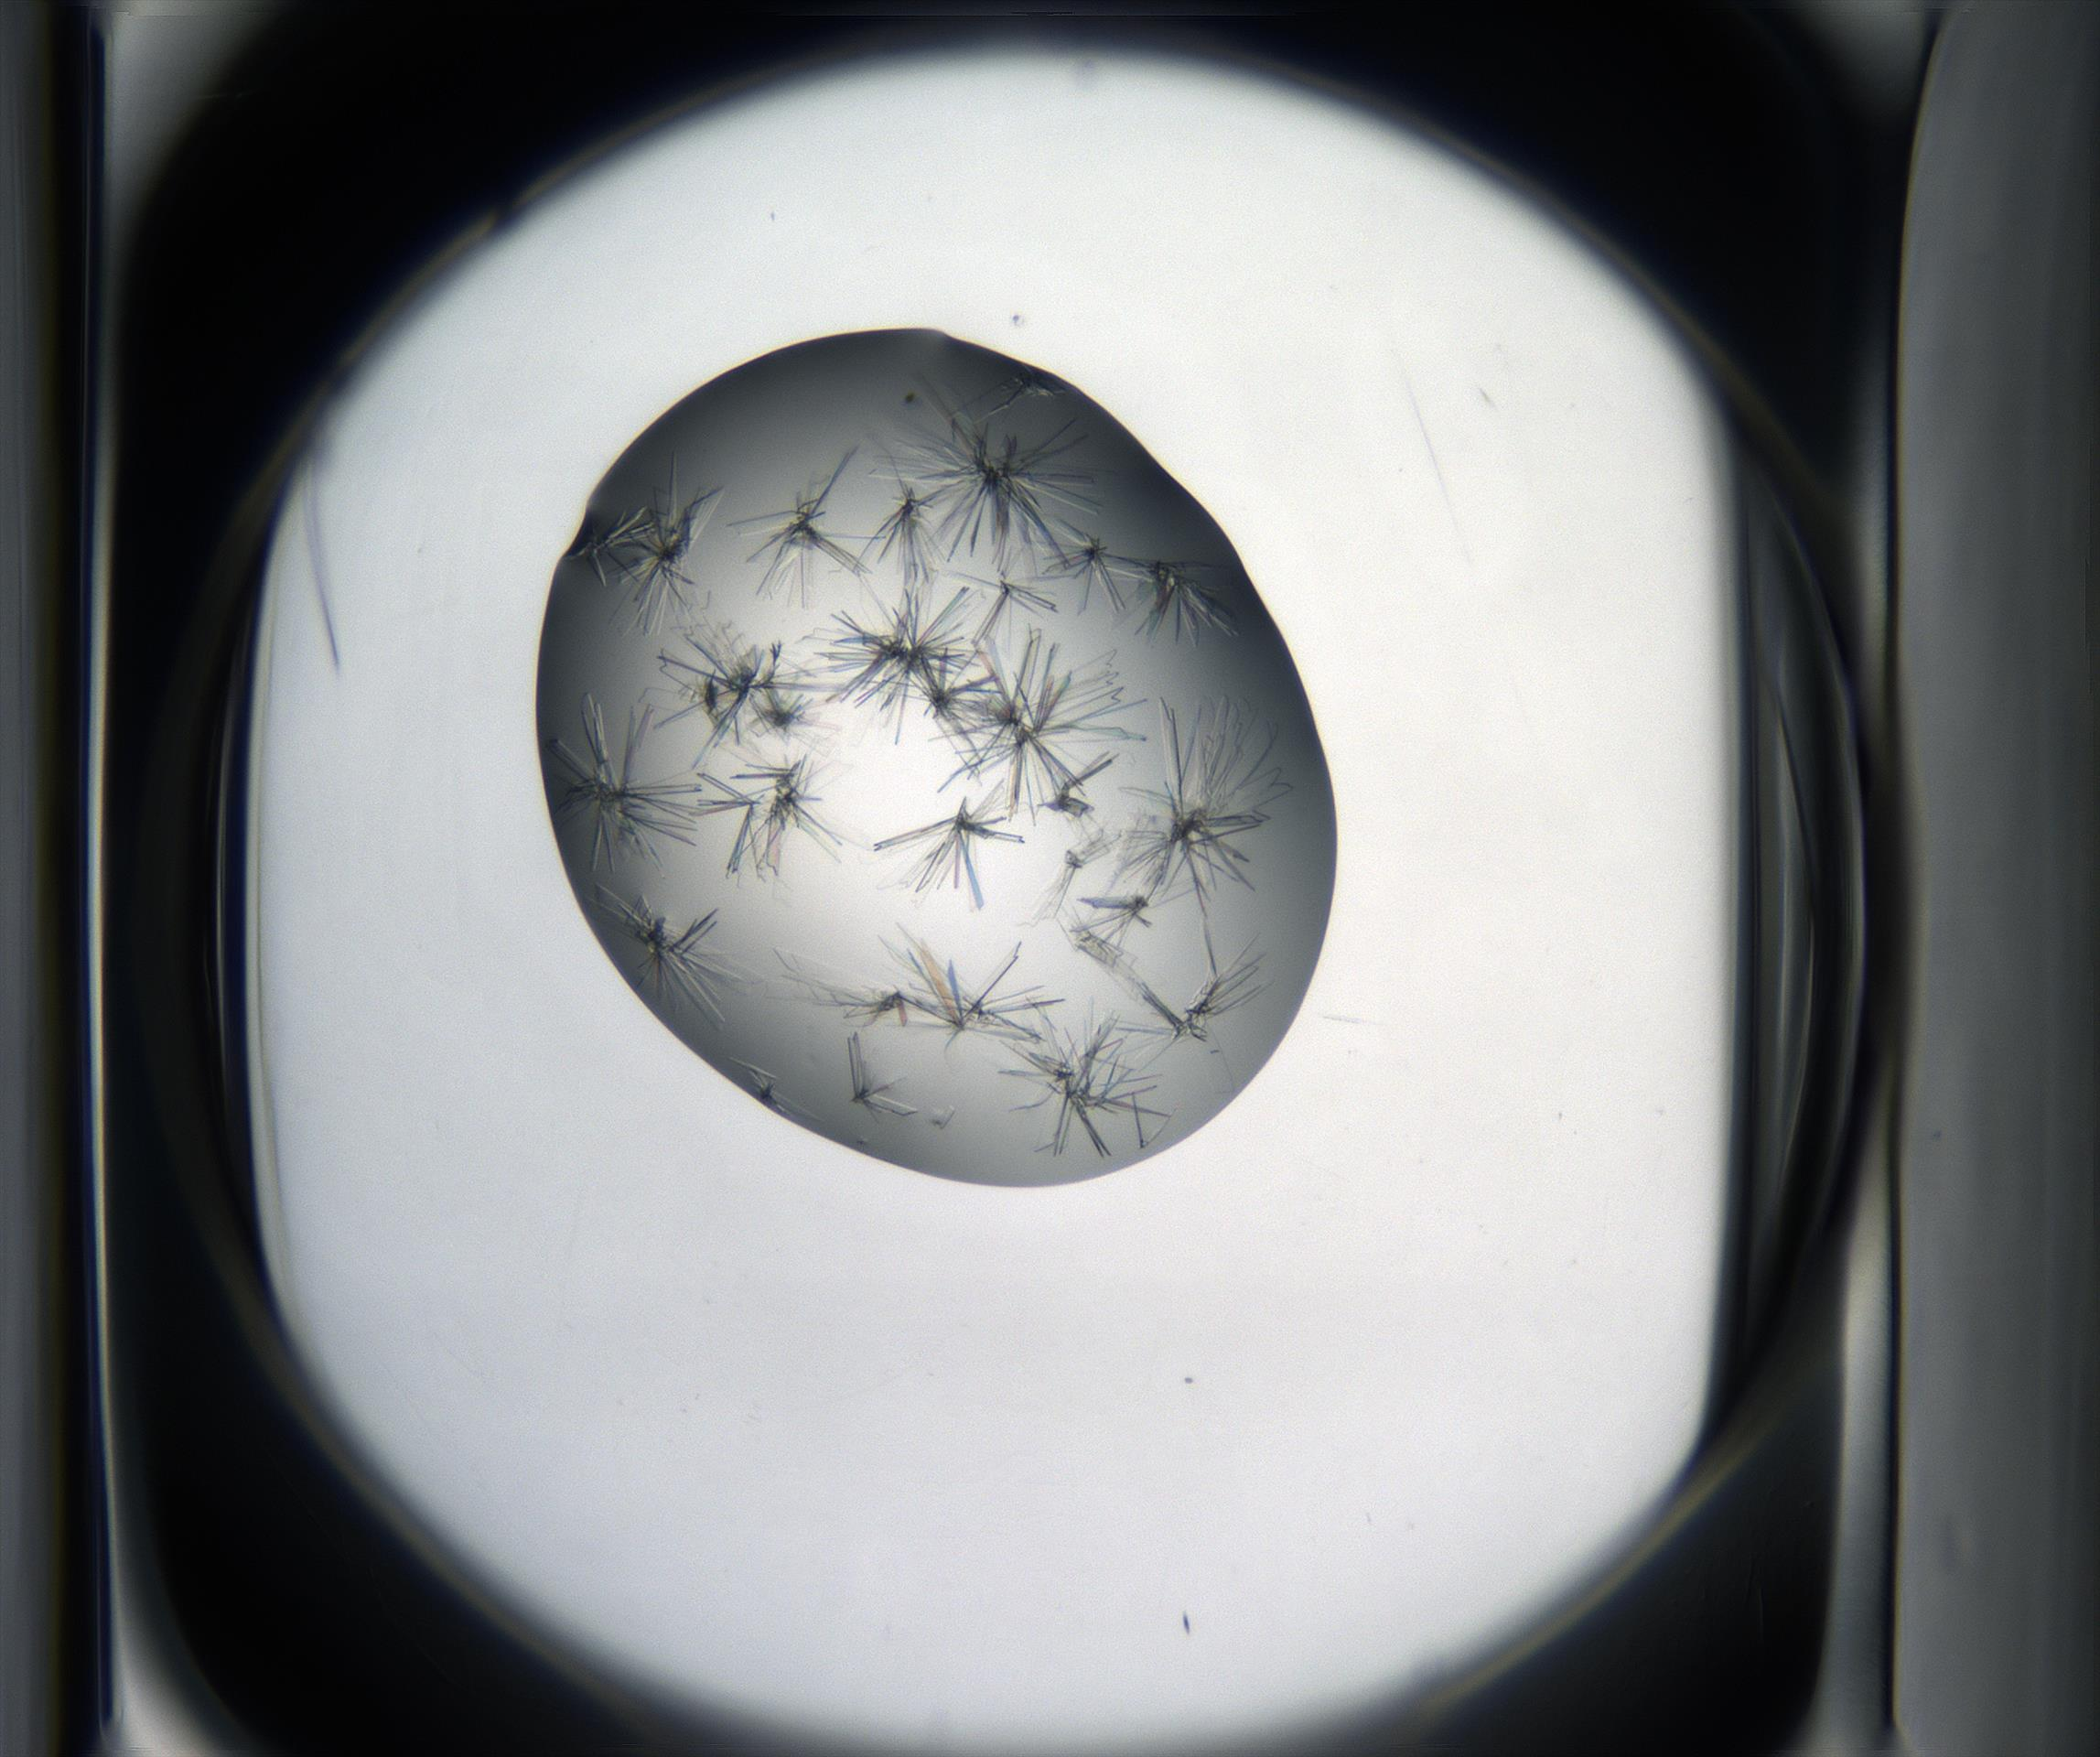
\includegraphics[width=\textwidth]{media/FORMULATRIX_SD30010708_4_07-10-2025_10_06_01_00_99_Vis}
            \end{subfigure}
            \begin{subfigure}[b]{0.24\textwidth}
                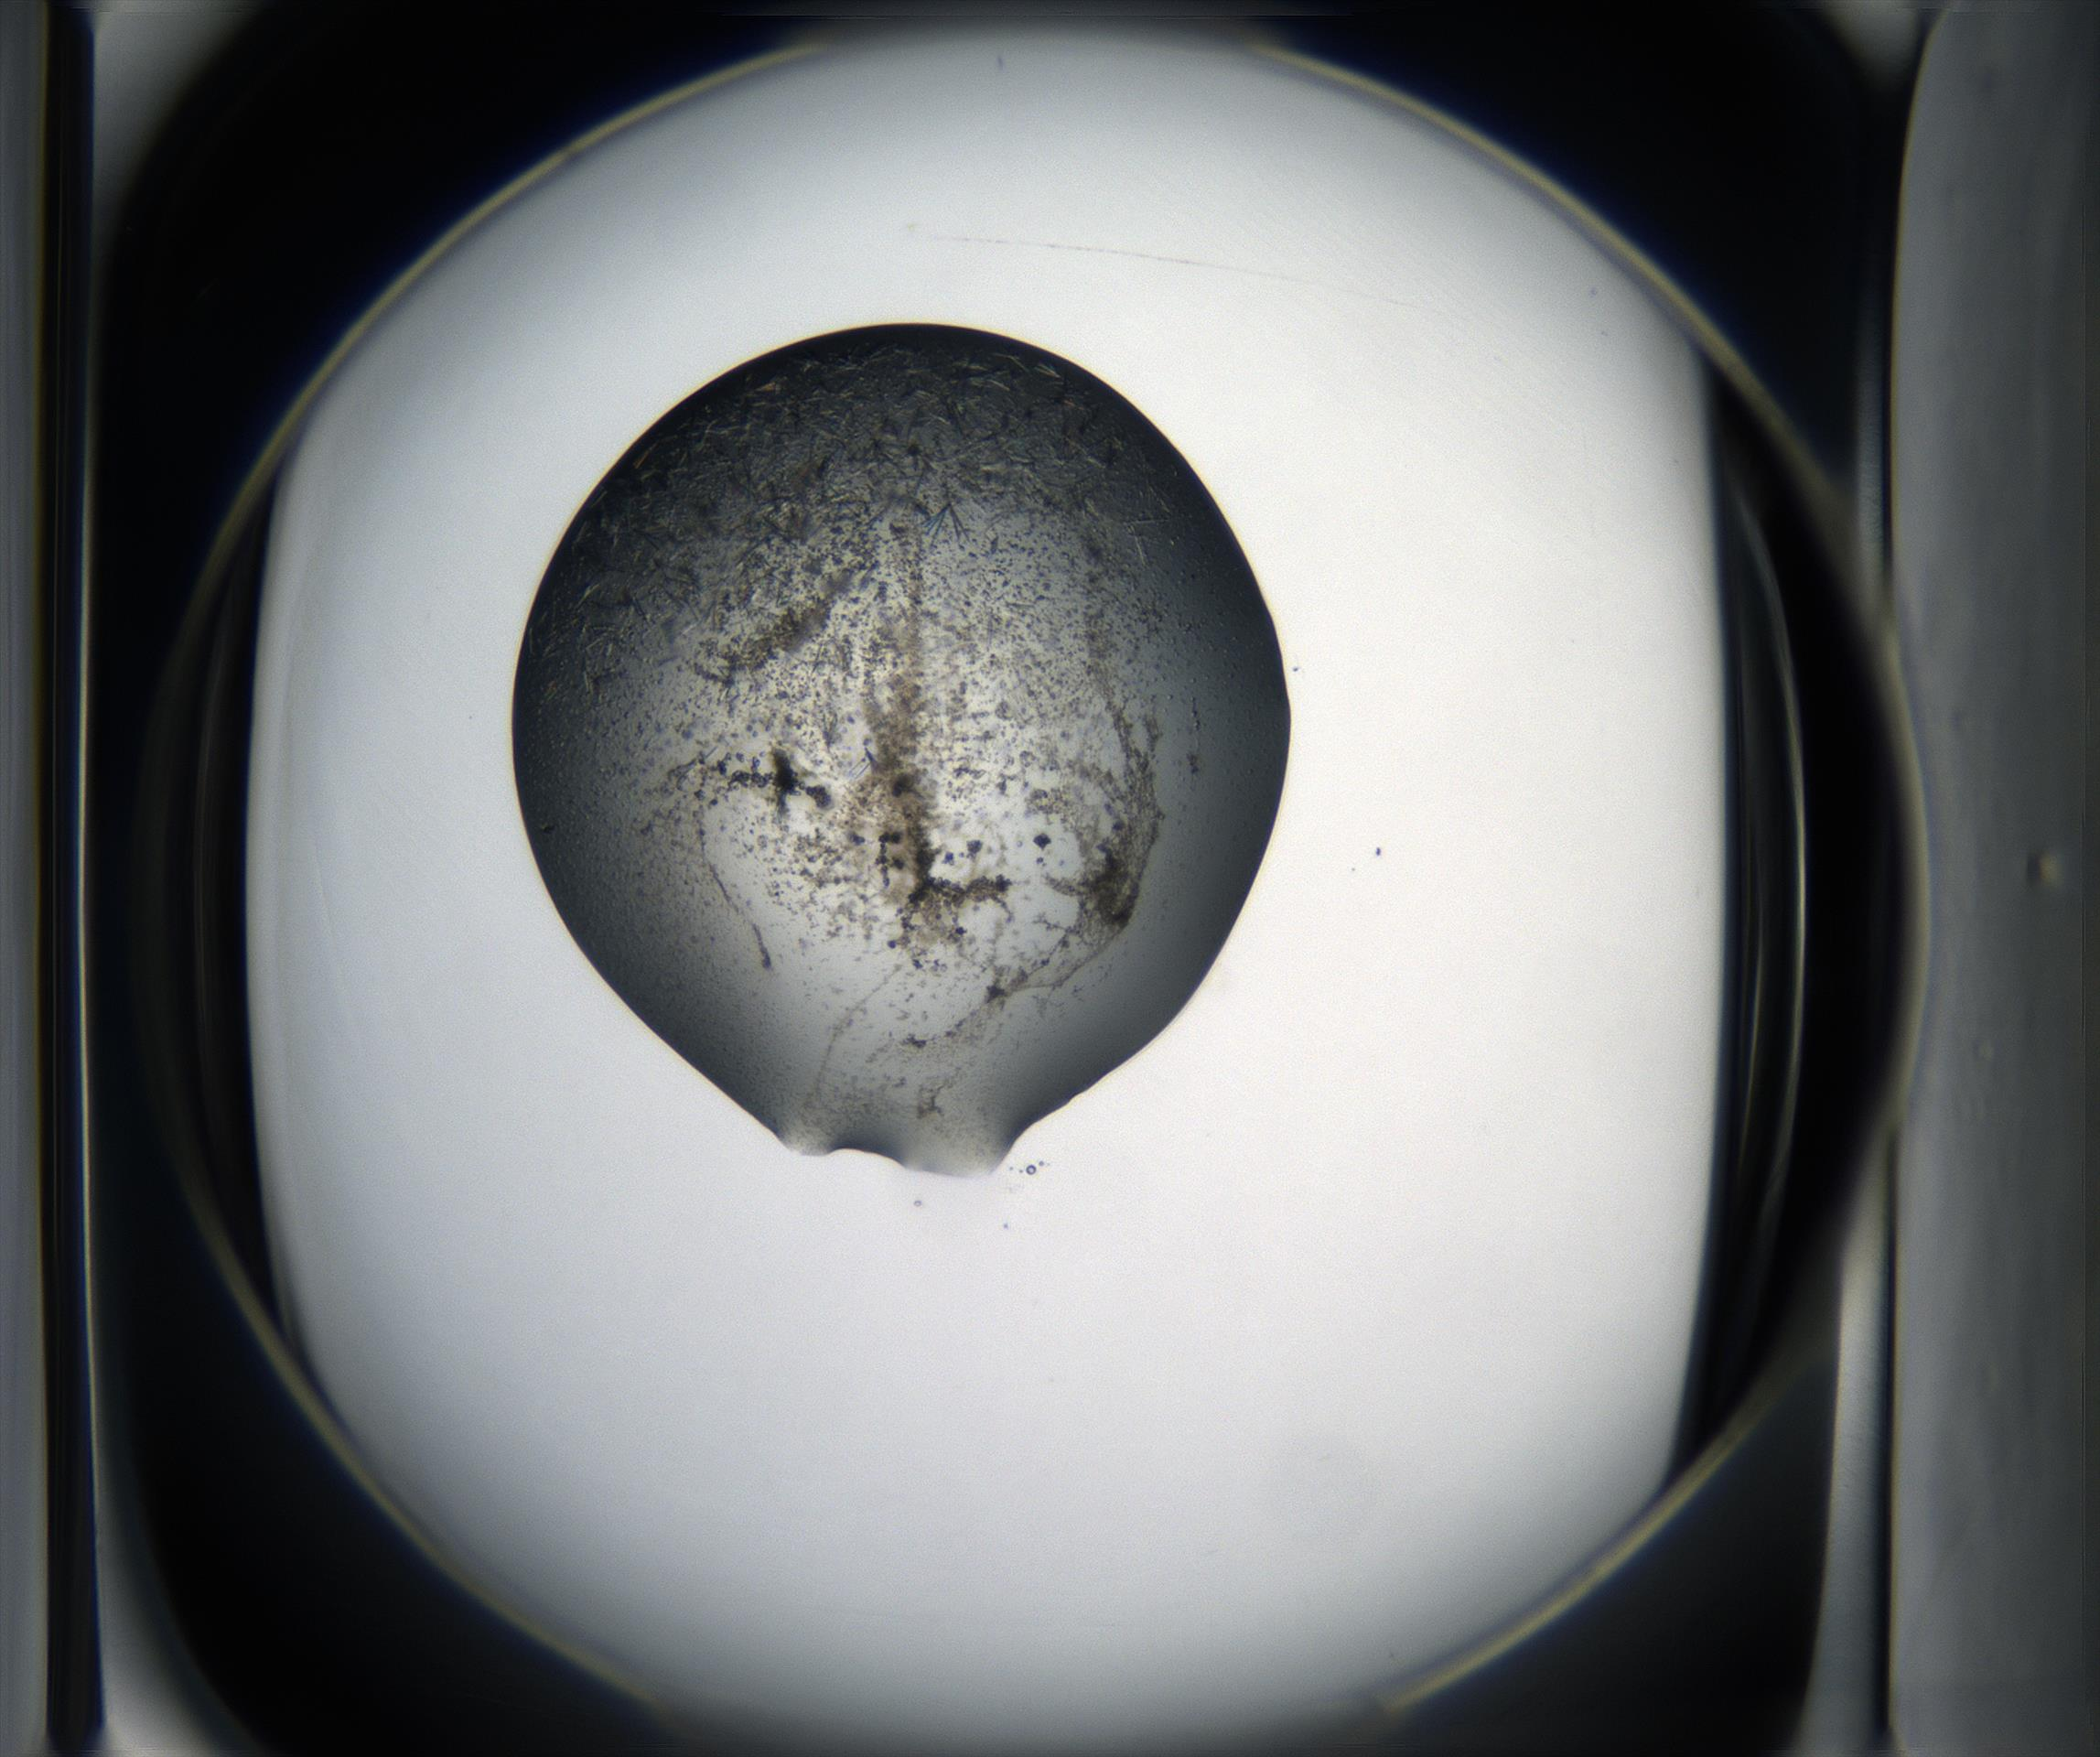
\includegraphics[width=\textwidth]{media/FORMULATRIX_SD30010708_4_07-10-2025_12_08_01_00_99_Vis}
            \end{subfigure}
            \begin{subfigure}[b]{0.24\textwidth}
                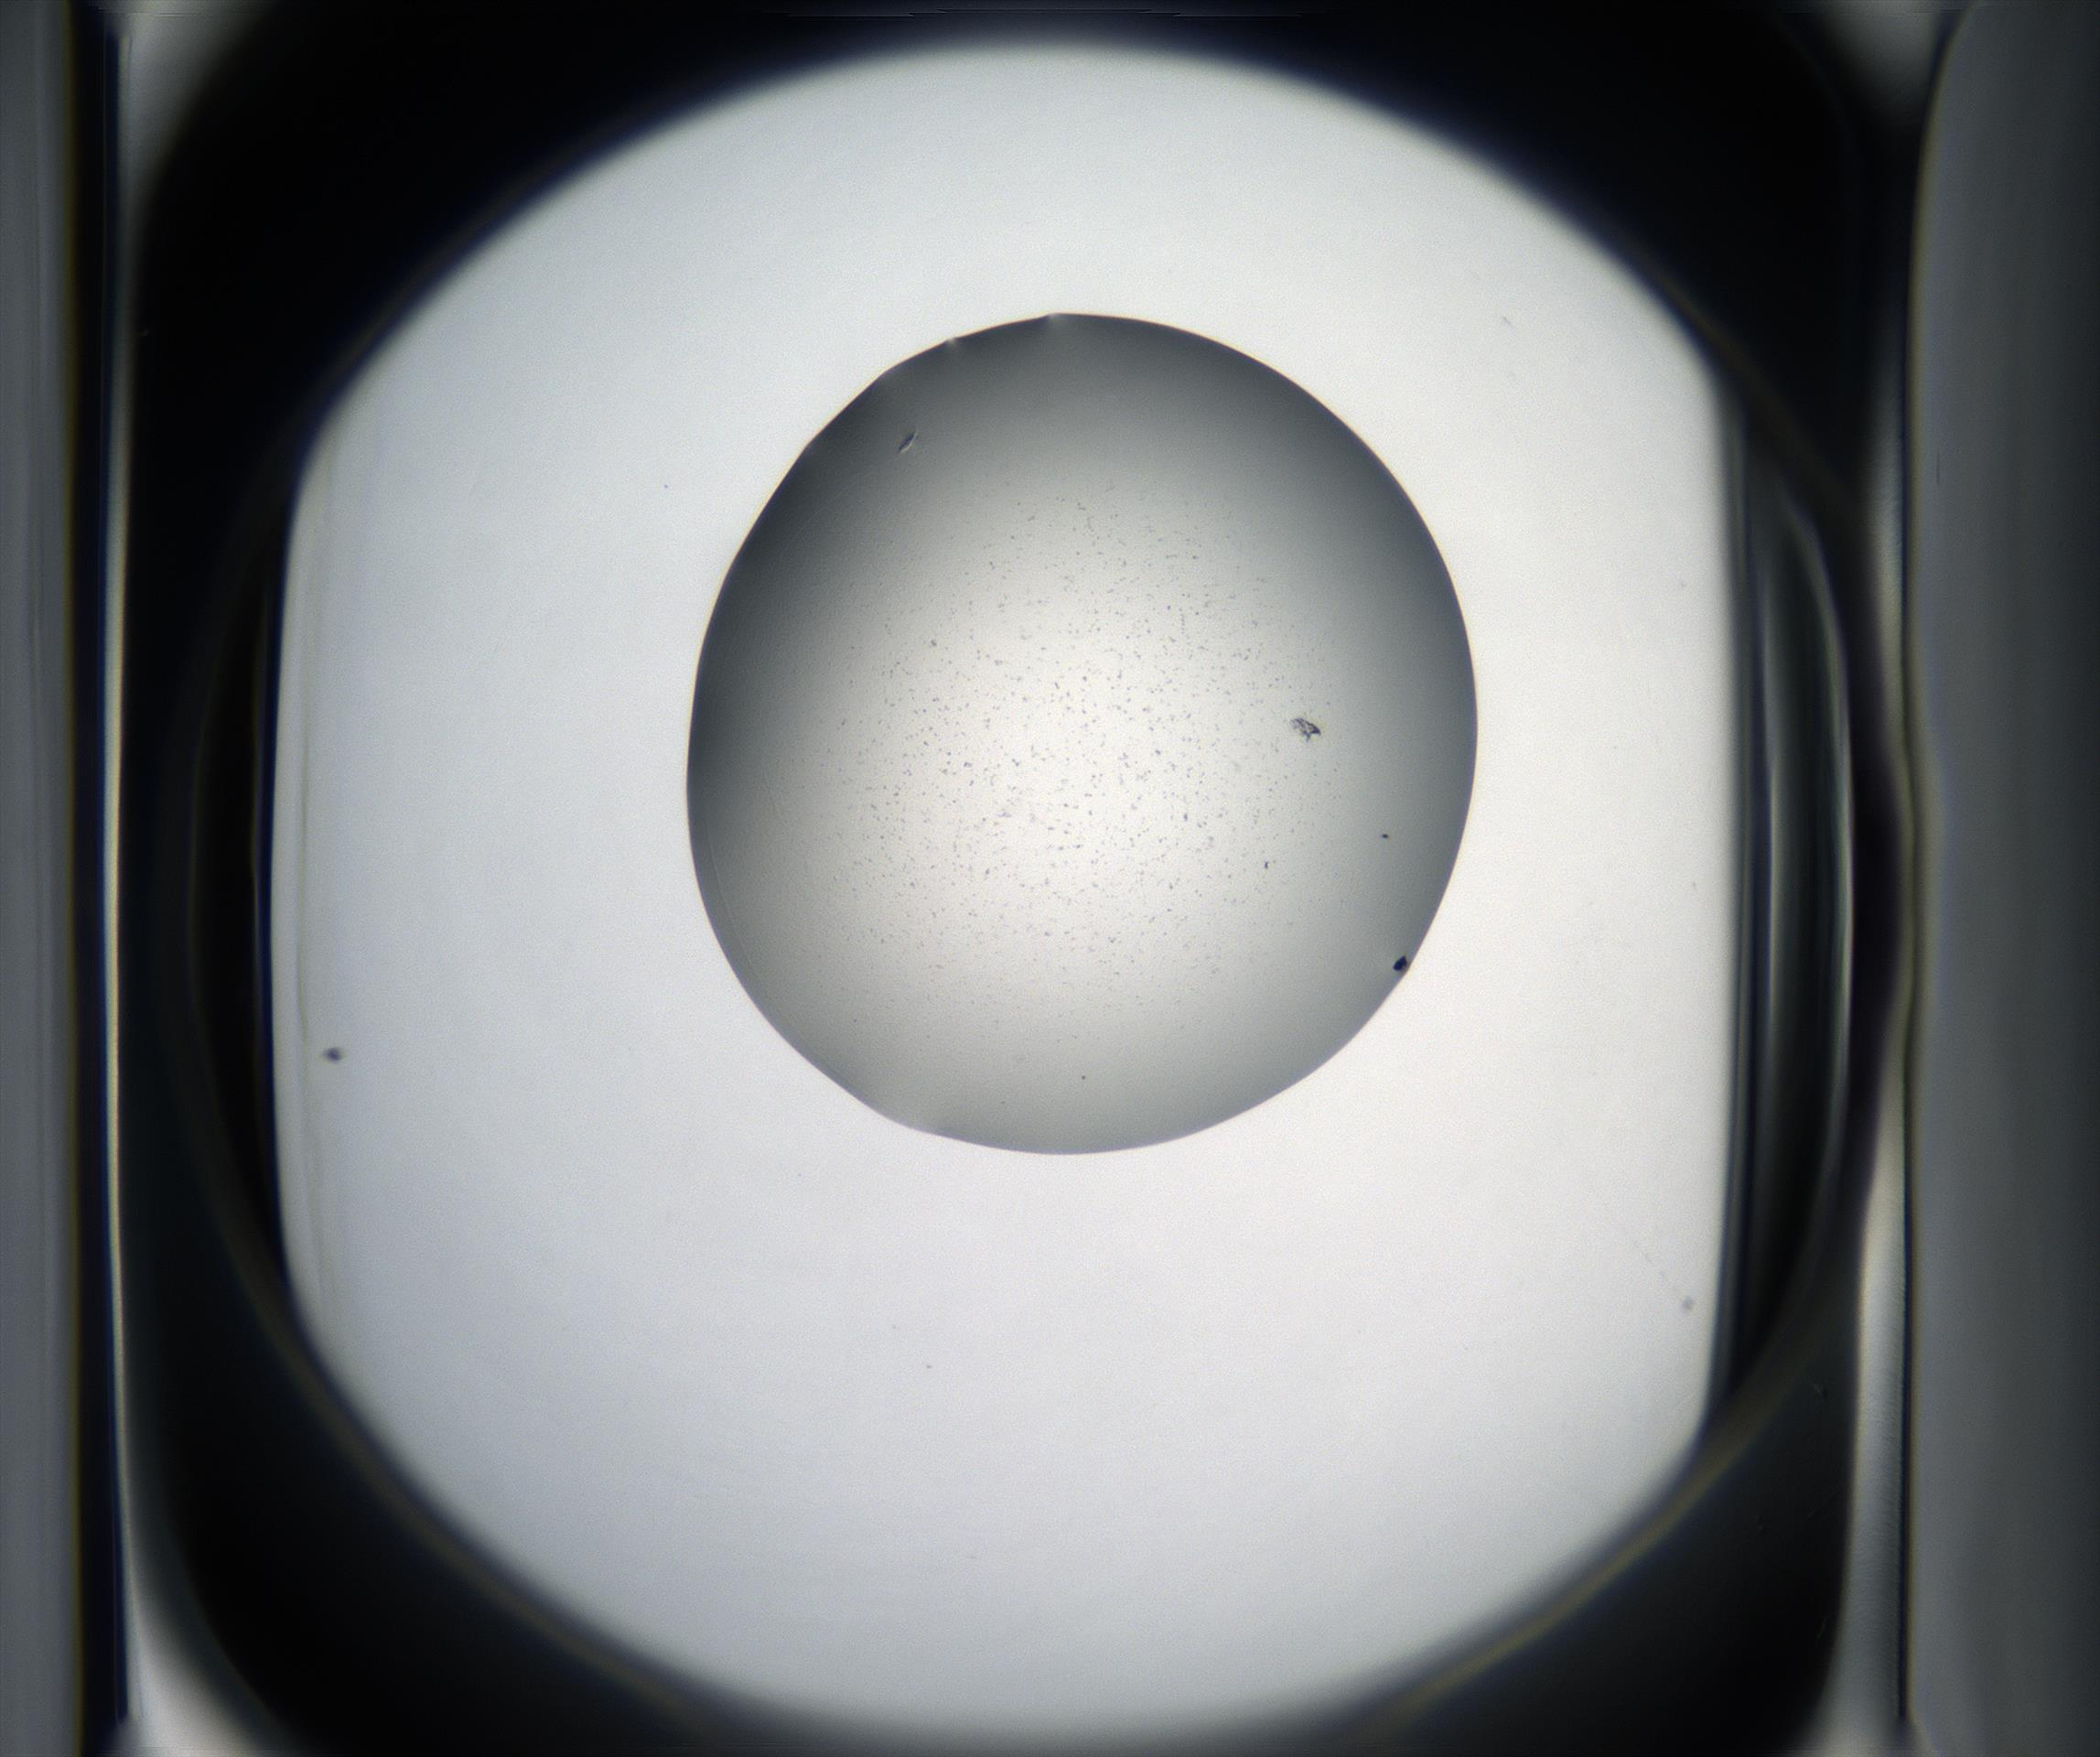
\includegraphics[width=\textwidth]{media/FORMULATRIX_SD30010708_4_07-10-2025_06_04_01_00_99_Vis}
            \end{subfigure}				
            \caption[\gls{crims} examples]{ 0.99, 0.97, 0.90, 0.3 $\rightarrow$ 0.99, 0.8, 0.1, 0}
            \label{fig:crystallization_drops_example}
        \end{figure}
        \vspace{-0.6cm}
        \begin{enumerate}
            \item Manual labeling (40k images) + expert annotations
            \item Training a CNN-based image scoring model on these labels (\textbf{98\% agreement})
            \item Manual validation of the model's predictions on uncertain cases  
            \item UV labels
        \end{enumerate} 

        \column{0.4\textwidth}
        \begin{itemize}
            \item \textbf{1.1\%} of conditions produced crystals {\tiny (cf. \ref{frame:crystallization_sucess})}
            \item \gls{crims} as a gold-standard test dataset
        \end{itemize}
        \begin{figure}[h]
            \centering
            \includegraphics[width=\textwidth]{media/uv_crystal.png}
            \label{fig:uv_imaging_example}
        \end{figure} 
    \end{columns}
\end{frame}

% only include, no negatives, high protein variance and parsing
\subsection{Protein Database}
\begin{frame}[shrink=10]{Protein Database}
    \begin{columns}[T]
        \column{0.5\textwidth}
        \begin{itemize}
            \item $>$220{,}000 entries
            \item Input: Sequence, Structure
            \item Label: 
                \begin{itemize}
                    \item pH, temperature {\tiny cf. \ref{frame:temperatureAndPh}, \ref{frame:enteredVsParsed}} 
                    \item free text, requires parsing {\tiny cf. \ref{frame:detailsExamples}, \ref{frame:dataOccurences}}
                    \item sparse {\tiny cf. \ref{frame:MissingPercentageCondition}} 
                \end{itemize}
            \item no negatives
            \item high protein variance
        \end{itemize}

        \column{0.5\textwidth}
        \vspace{-0.35cm}
        \begin{figure}
		\centering
		\includegraphics[width=0.5\linewidth]{Figures/proteinExample.png}
		\label{fig:ProteinExample}
	    \end{figure}
        \vspace{-0.5cm}
        {\small \texttt{Crystallization was carried out in sitting-drop vapor-diffusion setups with 1:1 mixtures of protein solution containing 0.7 mM Cko and 1.8 mM MnCl2 and reservoir solution containing 20\% PEG 3350 and 0.2 M Na2HPO4 , pH 9.5, VAPOR DIFFUSION, SITTING DROP, temperature 298K}}
    \end{columns}
\end{frame}

\subsection{Parsing}

\begin{frame}{Parsing Pipeline}
\centering
\begin{tikzpicture}[
    node distance=0.25cm,
    every node/.style={font=\scriptsize},
    step0/.style={
        draw,
        rounded corners,
        fill=uhhred!50,
        align=left,
        text width=8cm,
        inner sep=6pt
    },
    step1/.style={
        draw,
        rounded corners,
        fill=ukeblue!30,
        align=left,
        text width=8cm,
        inner sep=6pt
    },
    step2/.style={
        draw,
        rounded corners,
        fill=ukeblue!50,
        align=left,
        text width=8cm,
        inner sep=6pt
    },
    step3/.style={
        draw,
        rounded corners,
        fill=ukeblue!80,
        align=left,
        text width=8cm,
        inner sep=6pt
    },
    step4/.style={
        draw,
        rounded corners,
        fill=ukeblue!90,
        align=left,
        text width=8cm,
        inner sep=6pt
    },
    arrow/.style={thick, -{Latex[length=2mm]}}
]

\node[step0] (input) {%
\textbf{Free-text crystallization conditions}
};

\node[step1, below=of input] (parsing) {%
\textbf{1. Details parsing \& text normalization}

\begin{enumerate}\itemsep0pt
    \item Extract chemicals \& concentrations
    \item Extract pH \& temperature
\end{enumerate}
};

\node[step2, below=of parsing] (dict) {%
\textbf{2. Controlled vocabulary / compound dictionary}
\begin{enumerate}\itemsep0pt
    \item Canonicalize synonyms
    \item Map formulas and names
\end{enumerate}
};

\node[step3, below=of dict] (fuzzy) {%
\textbf{3. Fuzzy string matching}
\begin{enumerate}\itemsep0pt
    \item Reference set of frequent chemicals
    \item Levenshtein similarity with $> 90\%$ threshold 
    \item Manual false-positive filtering
\end{enumerate}
};

\node[step4, below=of fuzzy] (output) {%
\textbf{4. Output}
};

\draw[arrow] (input) -- (parsing);
\draw[arrow] (parsing) -- (dict);
\draw[arrow] (dict) -- (fuzzy);
\draw[arrow] (fuzzy) -- (output);

\end{tikzpicture}
\end{frame}

\subsection{Condition Analysis}
\begin{frame}{Condition Analysis}
    \begin{figure}[h!]
	\centering		
	\begin{subfigure}[b]{0.42\linewidth}
		\centering
		\includegraphics[width=\linewidth]{../msc-thesis-code/data/dataExploration/plots/nCompoundsDistribution}
		\label{fig:nCompoundsDistribution}
	\end{subfigure}
	\hspace{0.1cm}
	\begin{subfigure}[b]{0.55\linewidth}
		\centering
		\includegraphics[width=\linewidth]{../msc-thesis-code/data/dataExploration/plots/mostCommonchemicalCompounds_withConcentrationGiven}
		\label{fig:mostCommonChemicals}
	\end{subfigure}
	\caption[General Cocktail composition]{The number of compounds per cocktail and the most common chemical compounds in the dataset}
	\label{fig:cocktailSizeAndMostCommonCompounds}
\end{figure}
\end{frame}

